\chapter{MARCO TEÓRICO}

El marco teórico de este proyecto de investigación se centrará en los conceptos y técnicas fundamentales que subyacen en el algoritmo que se desarrollará. Este algoritmo integrará técnicas de aprendizaje profundo (Deep Learning), visión por computadora y SLAM (Simultaneous Localization and Mapping) para el monitoreo de granjas de jaulas de salmón.

\section{Aprendizaje Profundo (Deep Learning)}

El aprendizaje profundo es una sub categoría de la inteligencia artificial que se centra en algoritmos inspirados en la estructura y función del cerebro llamados redes neuronales artificiales. Estos algoritmos son capaces de aprender de grandes cantidades de datos y han demostrado ser extremadamente eficaces en muchas aplicaciones, incluyendo la visión por computadora, el procesamiento del lenguaje natural, y el reconocimiento del habla.

En este proyecto, se utilizará una arquitectura de red neuronal convolucional específica llamada Mask R-CNN con ResNET-101, RFP y DCN para la detección de huecos en las redes de las jaulas de salmón. Las redes neuronales convolucionales (CNNs) son una clase especial de redes neuronales que han demostrado ser muy eficaces en tareas de visión por computadora. 

\subsection{Mask R-CNN}

Mask R-CNN es un modelo utilizado para la detección y segmentación de objetos en imágenes. Está basado en Feature Pyramid Network (FPN) y una estructura de red neuronal ResNet101 \cite{matterport_maskrcnn_2017}. Esta técnica permite la segmentación de instancias, es decir, la identificación y clasificación de objetos individuales en una imagen. La segmentación de instancias es una tarea importante en la visión por computadora, ya que permite la identificación y clasificación de objetos individuales en una imagen. 


Se puede dividir en 2 etapas: generación de la región deseada (ROI), y clasificación y segmentación. La primera etapa es una arquitectura de tipo backbone CNN, donde se extrae las características (o features) de la imagen. La segunda etapa, obtiene los bounding boxes de la detección para luego extraer únicamente su forma \cite{cite:Zhang}. El output de este algoritmo se puede apreciar en la imagen \ref{fig:mask_crnn}.

\begin{figure} [!h]
    \begin{center}
    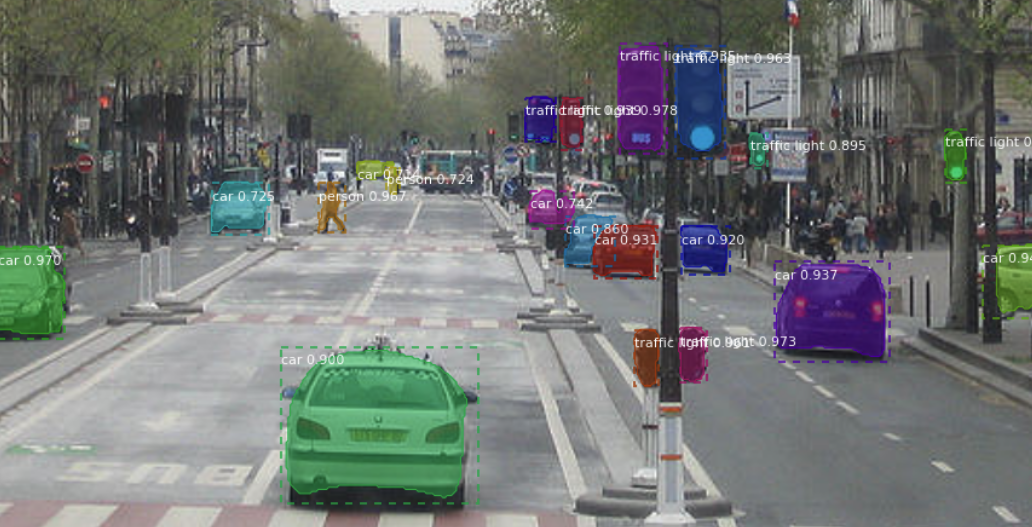
\includegraphics[height=6cm]{images/mask_crnn.png} 
    \caption{\label{fig:mask_crnn} Ejemplo de lo obtenido del método MASK CRNN en \cite{matterport_maskrcnn_2017}.}
    \end{center}
\end{figure}


\subsection{Redes residuales ResNET-101}

Las redes residuales (ResNet) son redes neuronales que se basan en el concepto de aprendizaje residual. Estas redes están compuestas por bloques de construcción que incluyen capas convolucionales y conexiones de atajo. La idea principal detrás de las ResNet es permitir que las redes sean más profundas sin sufrir degradación en el rendimiento. Esto se logra mediante la introducción de conexiones de atajo que saltan una o más capas, lo que permite que la información fluya directamente a través de la red. 

ResNet-101 es una variante específica de las redes residuales que consta de 101 capas. Esta arquitectura se destaca por utilizar bloques residuales como sus componentes principales. Cada bloque residual está compuesto por varias capas convolucionales y de activación que se organizan en una estructura en cascada. La salida de un bloque residual se convierte en la entrada del siguiente bloque. Sin embargo, lo que diferencia a las ResNet de otras arquitecturas es la introducción de conexiones de atajo o conexiones residuales \cite{cite:Kaiming}.

\subsection{Feature Pyramid Networks (FPN)}

Feature Pyramid Networks (FPN) es una arquitectura que ha demostrado una mejora significativa como un extractor de características genérico en varias aplicaciones, incluyendo la detección de objetos, segmentación semántica y segmentación de instancias. FPN está diseñada para abordar el desafío de detectar objetos en diferentes escalas en una imagen. El enfoque tradicional para la detección de objetos involucra el uso de un mapa de características de una sola escala, lo cual no es efectivo para detectar objetos de diferentes tamaños. FPN, por otro lado, construye una pirámide de características que posee una rica semántica en todos los niveles y se construye rápidamente a partir de una sola escala de imagen de entrada \cite{cite:Tsung}.

La arquitectura de FPN combina características de baja resolución y alta semántica con características de alta resolución y baja semántica a través de una vía descendente y conexiones laterales. Esto resulta en una pirámide de características que tiene una fuerte semántica en todas las escalas y puede ser utilizada para reemplazar pirámides de imágenes con características sin sacrificar el poder representativo, la velocidad o la memoria. El éxito de FPN en la detección de objetos resalta la importancia de utilizar redes neuronales convolucionales profundas para construir pirámides de características que puedan detectar eficazmente objetos en diferentes escalas.


\section{Visión por Computadora}

La visión por computadora es una disciplina que se centra en enseñar a las máquinas a 'ver' e interpretar imágenes y videos de la misma manera que los humanos. En este proyecto, se utilizarán técnicas de visión por computadora para identificar áreas de la red que están sucias y estimar el porcentaje total de suciedad. Parte de las herramientas usadas son distintos procedimientos de imágenes digitales, los cuales serán explicados con información extraída de \cite{cite:Gonzalez}.

\subsection{Método de Otsu}

El método de Otsu es una técnica de umbralización que se utiliza para convertir una imagen en escala de grises en una imagen binaria. Este método selecciona el umbral que minimiza la varianza intra clase de los píxeles de la imagen. En este proyecto, el método de Otsu se utilizará para segmentar la imagen de la red y facilitar la identificación de las áreas sucias.

\subsection{Histograma de Gradientes Orientados (HOG)}

El Histograma de Gradientes Orientados (HOG) es una técnica que se utiliza para la extracción de características en imágenes. Esta técnica cuenta las ocurrencias de los gradientes de intensidad de la imagen en direcciones orientadas. Los HOG son muy eficaces para la detección de formas y estructuras en las imágenes. En este proyecto, se utilizarán los HOG para identificar las áreas de la red que están sucias.


\section{SLAM Visual-Inercial-Presión}

SLAM (Simultaneous Localization and Mapping) es una técnica de Computer vision que permite a un robot mapear su entorno mientras se localiza en él. En este proyecto, se utilizará una versión de SLAM que combina datos de una cámara monocular, un sensor inercial (IMU) y un sensor de presión para la reconstrucción 3D de las granjas de jaulas de salmón. Para la explicación de este campo se extraerá información de \cite{cite:Gao} y \cite{cite:Ferrera}.

El SLAM visual-inercial es una variante de SLAM que utiliza datos de una cámara y un sensor inercial para estimar la trayectoria del robot y el mapa del entorno. Esta técnica es muy eficaz en entornos donde el GPS no está disponible o es poco fiable, como es el caso de las granjas de jaulas de salmón submarinas. La adición de un sensor de presión permite una estimación más precisa de la profundidad.